\documentclass[12pt,a4paper]{article}
\usepackage[utf8]{inputenc}
\usepackage[OT1]{fontenc}
\usepackage{amsmath}
\usepackage{amsfonts}
\usepackage{amssymb}
\usepackage{graphicx}
\usepackage{tikz}
\usepackage{pgfplotstable}
\usepackage{mathtext}

\usepackage[T1]{fontenc}
\usepackage[utf8]{inputenc}
\usepackage[english, bulgarian, russian]{babel}

\usepackage{tikz}
\usepackage{pgfplots}
\usepackage{indentfirst}
\usepackage[export]{adjustbox}
\usepackage{multirow}
\usepackage{geometry} \geometry{verbose,a4paper,tmargin=2cm,bmargin=2cm,lmargin=1.5cm,rmargin=1.5cm}

\graphicspath{{Images/}}
\usepackage[left=2cm,right=2cm,top=2cm,bottom=2cm]{geometry}
\usepackage{wrapfig}
\usepackage{setspace}
\usepackage{indentfirst}
\usepackage{subfigure}


\begin{document}

\begin{titlepage}
  \begin{center}
    \huge
    Московский Физико-технический Институт
    
    (Национальный исследовательский университет)
    \vspace{0.5cm}

   
    \vspace{0.25cm}
 
    \vfill
 
    \vfill

    \textsc{\bf{Отчет выполнении работы 2.2.6}}\\[3mm]
    
    {\LARGE Определение энергии активации по температурной зависимости вязкости жидкости}
  \bigskip
    \vfill
    
\end{center}
\vfill
\begin{flushright}

    Выполнили студентки 1 курса
    
    ФБМФ, группа Б06-103

    Попеску Полина
    
    
    Фитэль Алёна

\end{flushright}
\bigskip


\vfill

\begin{center}
  Долгопрудный, 2022 г.
\end{center}
\end{titlepage}

\section{Введение}

\textbf{Цель работы:} 1) измерение скорости падения шариков при разной температуре жидкости; 2) вычисление вязксоти жидкости по закону Стокса и расчет энергии активации.
	
\textbf{В работе используются:} стеклянный цилиндр с исследуемой жидкостью (глицерин); термостат; секундомер; горизонтальный компаратор; микроскоп; мелкие шарики (диаметром 1-2 мм).
	


\section{Теоретический материал}

По своим свойствам жидкости сходны как с газами, так и с твердыми телами. Подобно газам, жидкости принимают форму сосуда, в котором они находятся. Подобно твердым телам, они обладают сравнительно большой плотностью, с трудом поддаются сжатию.Двойственный характер свойств жидкостей связан с особенностями движения их молекул. В газах молекулы движутся хаотично, в их расположении отсутствует порядок. В кристаллических твердых
телах частицы колеблются около определенных положений равновесия -- узлов кристаллической решетки. В жидкостях, как и в кристаллах, каждая молекула находится в потенциальной яме электрического поля, создаваемого окружающими молекулами. Молекулы колеблются со средней частотой, близкой к частоте колебаний атомов в кристаллических телах. Глубина потенциальной ямы в жидкостях больше средней кинетической энергии колеблющейся молекулы, поэтому молекулы колеблются вокруг более или менее стабильных положений равновесия. Однако у жидкостей различие между этими двумя энергиями невелико, так что молекулы нередко выскакивают из своей потенциальной ямы и занимают место в другой. В отличие от твердых тел, жидкости обладают  рыхлой структурой. В них имеются свободные места  -- дырки, благодаря чему молекулы могут перемещаться, покидая свое место и занимая одну из соседних дырок. Таким образом, молекулы медленно перемещаются внутри жидкости, пребывая часть времени около определенных мест равновесия и образуя картину меняющейся со временем пространственной решетки. На современном языке принято говорить, что в жидкости присутствует ближний, но не дальний порядок, расположение молекул упорядочено в небольших объемах, но порядок перестает замечаться при увеличении расстояния.

Отмеченный характер движения молекул объясняет как медленность диффузии в жидкостях, так и большую (по сравнению с газами) их вязкость. В газах вязкость объясняется происходящим при тепловом движении молекул переносом количества направленного движения. В жидкостях такие переходы существенно замедлены. Количество молекул, имеющих энергии больше W, в соответствии с формулой Больцмана экспоненциально зависит от W. Температурная зависимость вязкости жидкости выражается формулой :

\begin{equation}
\eta \approx Ae^{\frac{W}{kT}}
\label{eq:viscosity}
\end{equation}


Из данной формулы следует, что при повышении температуры вязкость должна резко понижаться. Если построить на графике логарифм вязкости lnη в зависимости от 1/T, должна получиться прямая линия, по угловому коэффициенту которой можно получить энергию активации молекулы исследуемой жидкости: 
\begin{equation}
W=k\frac{\text{d}(ln\eta)}{\text{d}(1/T)}
\label{eq:formula_for_graph}
\end{equation}
Для исследования температурной зависимости вязкости жидкости в данной работе используется метод Стокса, основанный на измерении скорости свободного падения шарика в жидкости. Суть его заключается в следующем.

На всякое тело, двигающееся в вязкой жидкости, действует сила сопротивления. В общем случае величина этой силы зависит от многих факторов: от вязкости жидкости, от формы тела, от характера обтекания и т. д. Стоксом было получено строгое решение задачи о ламинарном обтекании шарика безграничной жидкостью. В этом случае сила сопротивления F определяется формулой

\begin{equation}
F = 6\pi \eta rv
\label{eq:Stock's_force}
\end{equation}


где $\eta$ - вязкость жидкости, $v - $ скорость шарика, $r - $ радиус шарика.

Рассматривая свободное падение шарика в вязкой жидкости, получаем уравнение:

\begin{equation}
Vg\left(\rho - \rho_{\text{ж}}\right) - 6\pi \eta rv = V\rho \frac{dv}{dt}
\label{eq:Newton_second_law_for_ball}
\end{equation}


Решая данное уравнение относительно скорости, получаем:

\begin{equation}
v\left(t\right) = v_{\text{уст}} - \left[v_{\text{уст}} - v\left(0\right)\right]e^{\frac{-t}{\tau}}
\label{eq:velocity_equation}
\end{equation}


\begin{equation}
v_{\text{уст}} = \frac{2}{9}gr^{2}\frac{\rho - \rho_{\text{ж}}}{\eta}
\label{eq:velocity_ust_equation}
\end{equation}


\begin{equation}
\tau = \frac{2}{9}\frac{r^{2}\rho}{\eta}
\end{equation}


\section{Экспериментальная установка}

	Для измерений используется стеклянный цилиндрчиеский сосуд B, наполненный исследуемой жидкостью (глицерин). Диаметр сосуда $\approx 3$ см, длина $\approx 40$ см. На стенках сосуда нанесены две метки на некотором расстоянии друг от друга. Верхняя метка должна располагаться ниже уровня жидкости с таким расчетом, чтобы скорость шарика к моменту прохождения этой метки успевала установиться. Измеряя расстояние между метками с помощью линейки, а время падения с помощью секундомера, определяют скорость шарика vуст. Сам сосуд B помещен в рубашку D, омываемую водой из термостата. При работающем термостате температура воды в рубашке D, а потому и температура жидкости 12 равна температуре воды в термостате.
	
	Схема прибора (в разрезе) показана на рис.~\ref{ris:ustanovka}.


\begin{figure}[h!]
	\center{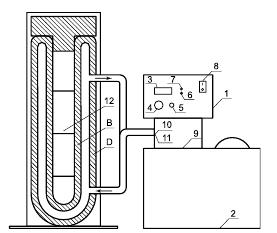
\includegraphics[scale=1.2]{Scem_of_facility.jpg}}
	\label{ris:ustanovka}
\end{figure}

\newpage

\section{Обработка результатов измерений}


\begin{enumerate}

\item Параметры установки: плотность стекла -- $2500$ кг/м$^3$, плотность стали -- $7800$ кг/м$^3$. Расстояния между метками $L_1 = L_2 = 10 \pm 0,05$ см

Погрешности:

$\Delta r = 0.05 $ мм, $\Delta t = 0.1$ с, $\Delta T = 1 $ К, $\Delta l = 0.005$ м

Соответствие температуры и плотности глицерина, определенные по графику:

\begin{table}[h!]
\centering
	\caption{Соответствие температуры плотности глицерина}

\begin{tabular}{|c|c|}
\hline
\multicolumn{1}{|l|}{t, $^\circ C$} & \multicolumn{1}{l|}{$\rho_{гл}$, кг/м$^3$} \\ \hline
23,0                         & 1259                             \\ \hline
30,4                       & 1255                             \\ \hline
38,2                       & 1252                             \\ \hline
46,4                       & 1248                             \\ \hline
55,0                         & 1244                             \\ \hline
\end{tabular}
\end{table}

\item Измерим установившиеся скорости падения шариков и вычислим вязкость по формуле (\ref{eq:velocity_equation}). Выполним измерения для 5 значений температур в интервале от комнатной до 55$^{\circ}$.

Погрешности для расчетов:

$\Delta V_{уст} = V_{уст} \cdot \sqrt{ \left(\frac{\Delta t}{t}\right)^2 + \left(\frac{\Delta l}{l}\right)^2  }$

$\Delta \eta = \eta \cdot \sqrt{ \left(\frac{2 \Delta r}{r}\right)^2 + \left(\frac{\Delta V_{уст} }{V_{уст} }\right)^2  }$

\begin{table}[h!]
\centering
	\caption{Результаты измерений для стеклянного шарика}

\begin{tabular}{|c|c|c|c|c|c|c|c|c|c|}
\hline
\multicolumn{1}{|l|}{t, $^\circ C$} & \multicolumn{1}{l|}{$r_ш$, м} & \multicolumn{1}{l|}{$t_1$} & \multicolumn{1}{l|}{$t_2$} & \multicolumn{1}{l|}{$V_{уст1}$, м/с} & \multicolumn{1}{l|}{$V_{уст2}$, м/с} & \multicolumn{1}{l|}{$\eta_1$, кг/(м*с)} & \multicolumn{1}{l|}{$\eta_2$, кг/(м*с)} & \multicolumn{1}{l|}{$\sigma ln(\eta _1)$} & \multicolumn{1}{l|}{$\sigma ln(\eta _2)$} \\ \hline
23,0                         & 0,0011                      & 28,4                    & 28,8                    & 0,00352                          & 0,00347                          & 0,93                              & 0,94                              & 0,08                     & 0,09                                             \\ \hline
23,0                         & 0,00105                     & 29,0                      & 29,0                      & 0,00345                          & 0,00345                          & 0,87                              & 0,87                              & 0,08                     & 0,08                                             \\ \hline
30,4                       & 0,001                       & 18,0                      & 18,4                    & 0,00556                          & 0,00543                          & 0,49                              & 0,50                              & 0,05                     & 0,05                                             \\ \hline
30,4                       & 0,00095                     & 18,6                    & 18,9                    & 0,00538                          & 0,00529                          & 0,46                              & 0,46                              & 0,05                     & 0,05                                             \\ \hline
38,2                       & 0,001                       & 9,2                     & 9,0                       & 0,01087                          & 0,01111                          & 0,25                              & 0,24                              & 0,03                     & 0,02                                             \\ \hline
38,2                       & 0,001                       & 9,3                     & 9,0                       & 0,01075                          & 0,01111                          & 0,25                              & 0,24                              & 0,03                     & 0,02                                             \\ \hline
46,4                       & 0,001                       & 5,6                     & 6,1                     & 0,01786                          & 0,01639                          & 0,15                              & 0,17                              & 0,02                     & 0,02                                             \\ \hline
46,4                       & 0,0012                      & 5,5                     & 6,2                     & 0,01818                          & 0,01613                          & 0,22                              & 0,24                              & 0,02                     & 0,02                                             \\ \hline
55,0                         & 0,0012                      & 3,6                     & 3,0                       & 0,02778                          & 0,03333                          & 0,14                              & 0,12                              & 0,01                     & 0,01                                             \\ \hline
55,0                         & 0,001                       & 3,2                     & 3,5                     & 0,03125                          & 0,02857                          & 0,09                              & 0,10                              & 0,01                     & 0,01                                             \\ \hline
\end{tabular}
\end{table}

\newpage 
	
\begin{table}[h!]
\centering
	\caption{Результаты измерений для стального шарика}

\begin{tabular}{|c|c|c|c|c|c|c|c|c|c|}
\hline
\multicolumn{1}{|l|}{t, $^\circ C$} & \multicolumn{1}{l|}{$r_ш$, м} & \multicolumn{1}{l|}{$t_1$} & \multicolumn{1}{l|}{$t_2$} & \multicolumn{1}{l|}{$V_{уст1}$, м/с} & \multicolumn{1}{l|}{$V_{уст2}$, м/с} & \multicolumn{1}{l|}{$\eta_1$, кг/(м*с)} & \multicolumn{1}{l|}{$\eta_2$, кг/(м*с)} & \multicolumn{1}{l|}{$\sigma ln(\eta _1)$} & \multicolumn{1}{l|}{$\sigma ln(\eta _2)$} \\ \hline
23,0                         & 0,0004                      & 42,4                    & 42,4                    & 0,00236                          & 0,00236                          & 0,97                              & 0,97                              & 0,24                       & 0,24                                               \\ \hline
23,0                         & 0,0004                      & 38,6                    & 38,4                    & 0,00259                          & 0,00260                          & 0,88                              & 0,88                              & 0,22                       & 0,22                                               \\ \hline
30,4                       & 0,0004                      & 17,0                      & 17,4                    & 0,00588                          & 0,00575                          & 0,39                              & 0,40                              & 0,10                       & 0,10                                               \\ \hline
30,4                       & 0,00045                     & 17,4                    & 18,2                    & 0,00575                          & 0,00549                          & 0,50                              & 0,53                              & 0,11                       & 0,12                                               \\ \hline
38,2                       & 0,0004                      & 11,9                    & 12,2                    & 0,00840                          & 0,00820                          & 0,27                              & 0,28                              & 0,07                       & 0,07                                               \\ \hline
38,2                       & 0,00045                     & 11,2                    & 11,9                    & 0,00893                          & 0,00840                          & 0,32                              & 0,34                              & 0,07                       & 0,08                                               \\ \hline
46,4                       & 0,00045                     & 6,0                       & 6,0                       & 0,01667                          & 0,01667                          & 0,17                              & 0,17                              & 0,04                       & 0,04                                               \\ \hline
46,4                       & 0,00045                     & 6,3                     & 6,5                     & 0,01587                          & 0,01538                          & 0,18                              & 0,19                              & 0,04                       & 0,04                                               \\ \hline
55,0                         & 0,00035                     & 5,5                     & 6,1                     & 0,01818                          & 0,01639                          & 0,10                              & 0,11                              & 0,03                       & 0,03                                               \\ \hline
55,0                         & 0,0004                      & 3,4                     & 3,4                     & 0,02941                          & 0,02941                          & 0,08                              & 0,08                              & 0,02                       & 0,02                                               \\ \hline
\end{tabular}
\end{table}

\item Для каждого из опытов вычислим значение числа Рейнольдса $Re$, оценим время релаксации $\tau$ и путь релаксации $S$.

\begin{table}[h!]
\centering
	\caption{Стеклянный шарик}

\begin{tabular}{|c|c|c|c|}
\hline
\multicolumn{1}{|l|}{$t, С^\circ$} & \multicolumn{1}{l|}{$Re$} & \multicolumn{1}{l|}{$\tau$, c} & \multicolumn{1}{l|}{$S$, мм} \\ \hline
23,0                         & 0,00510                 & 0,00071                   & 0,00247                    \\ \hline
23,0                         & 0,00527                 & 0,00071                   & 0,00244                    \\ \hline
30,4                       & 0,01365                 & 0,00111                   & 0,00604                    \\ \hline
30,4                       & 0,01362                 & 0,00108                   & 0,00573                    \\ \hline
38,2                       & 0,05678                 & 0,00227                   & 0,02520                    \\ \hline
38,2                       & 0,05678                 & 0,00227                   & 0,02520                    \\ \hline
46,4                       & 0,12281                 & 0,00333                   & 0,05467                    \\ \hline
46,4                       & 0,09907                 & 0,00328                   & 0,05292                    \\ \hline
55,0                         & 0,42044                 & 0,00676                   & 0,22532                    \\ \hline
55,0                         & 0,37068                 & 0,00579                   & 0,16554                    \\ \hline
\end{tabular}
\end{table}


\begin{table}[h!]
\centering
	\caption{Стальной шарик}
\begin{tabular}{|c|c|c|c|}
\hline
\multicolumn{1}{|l|}{$t, С^\circ$} & \multicolumn{1}{l|}{$Re$} & \multicolumn{1}{l|}{$\tau$, c} & \multicolumn{1}{l|}{$S$, мм} \\ \hline
23,0                         & 0,00123                 & 0,00029                   & 0,00068                    \\ \hline
23,0                         & 0,00150                 & 0,00032                   & 0,00082                    \\ \hline
30,4                       & 0,00726                 & 0,00070                   & 0,00401                    \\ \hline
30,4                       & 0,00590                 & 0,00067                   & 0,00367                    \\ \hline
38,2                       & 0,01472                 & 0,00099                   & 0,00815                    \\ \hline
38,2                       & 0,01376                 & 0,00102                   & 0,00857                    \\ \hline
46,4                       & 0,05390                 & 0,00202                   & 0,03369                    \\ \hline
46,4                       & 0,04593                 & 0,00187                   & 0,02871                    \\ \hline
55,0                         & 0,06680                 & 0,00199                   & 0,03257                    \\ \hline
55,0                         & 0,18813                 & 0,00357                   & 0,10485                    \\ \hline
\end{tabular}
\end{table}

Число Рейнольдса для всех случаев получилось очень мало, следовательно, течение можно считать ламинарным.

Время релаксации меньше времени прохождения шарика до первой отметки, следовательно, движение можно считать установившемся.

Таким образом, формула Стокса может быть применена.


\item Построим график зависимости $ln \eta$ от $1/T$.

\begin{figure}[h!]
	\center{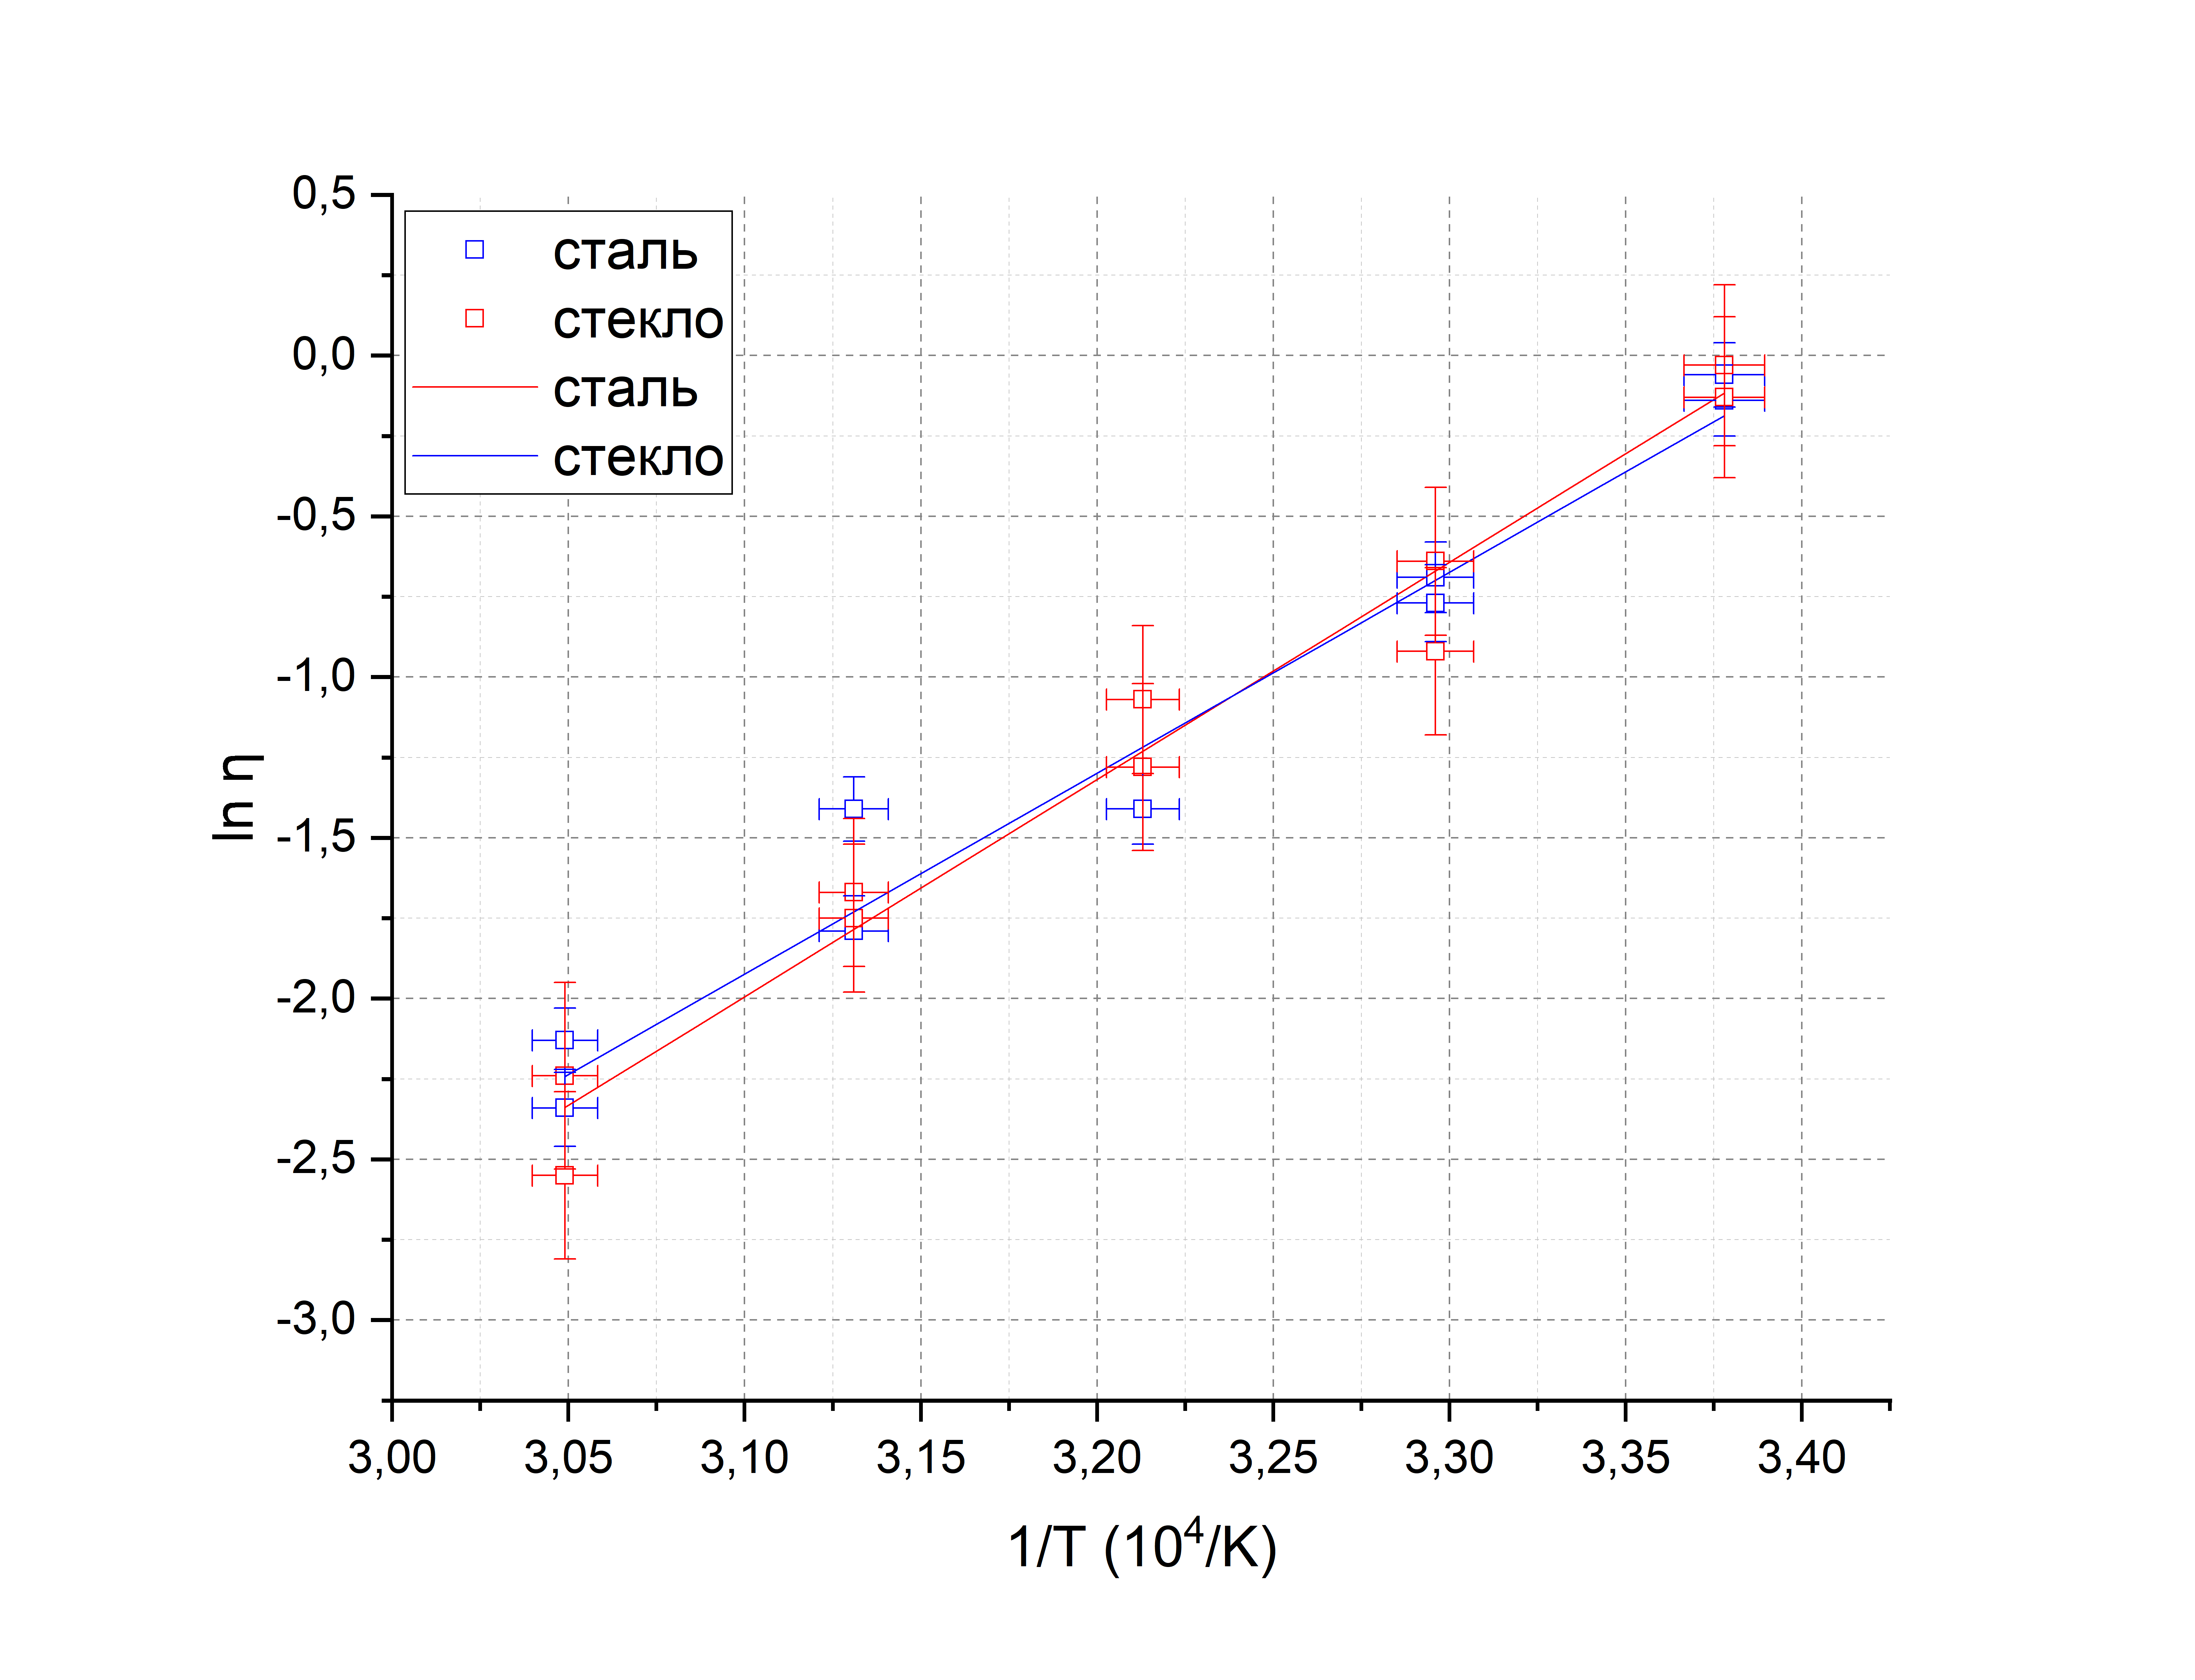
\includegraphics[scale=0.3]{graph226_1.png}}
\end{figure}

Наклон графика -- величина $W/k$. Для стеклянного шарика получим: $k_{стекло} = (6755 \pm 456)$, $W_{стекло} = (93.3 \pm 6.3) \cdot 10^{-20} \: Дж/моль$. Для стального: $k_{сталь} = (6246 \pm 393)$, $W_{сталь} = (86.2 \pm 5.4) \cdot 10^{-20} \: Дж/моль$.

Тогда итоговая энергия активации $$W=(89,8 \pm 5,9) \cdot 10^{-20} \: Дж/моль$$

\section{Вывод}

В данной работе была проверена справедливость формулы Стокса. Были вычислены числа Рейнольдса для движения шарика в вязкой жидкости, время релаксации и путь. На основе их величин было определено, что течение можно считать ламинарным, движение шарика - установившемся.

Была определена энергия активации глицерина $W = (89,8 \pm 5,9) \cdot 10^{-20} \: Дж/моль$.

\end{enumerate}

\end{document}
